\chapter{Introduction}

\section{Background}
Capacitive touchscreens are one of the most profound interaction interfaces on modern devices. Benefit from the sensitivity and robustness of capacitive touchscreen, it is able to provide seamless, intuitive interaction between users and digital media. Furthermore, comparing with resistive touchscreen, the possibility of multitouch enabled by capacitive touchscreen as well as the unbreakable freature makes it a dominance in the touchscreen market. However, capacitive screen is still relatively expensive comparing with resistive touchscreen. Though manufactures launched various different large-scale capacitive-screen products such as touchscreen wall, touchscreen table, touchscreen board, etc ~\ref{fig:touchscreen-products}, the price of these products are unaffordable to ordinary people, due to the cost of capacitive touchscreen per unit area. As the most affordable touchscreen products, smartphone's touch interface is still limited to the area where touch sensors are embedded, constraining natural user interactions to the surfaces of these smart devices. Therefore, simply scaling touchscreens to large surfaces and everyday objects is expensive and challenging, which limits its wider adoption in the Internet of Things applications. How to scale the sensing capability of small capacitive touchscreen to larger area in a low-cost manner to enable large-scale touch interactions has become a popular research topic in the field of Human Computer Interaction.

\begin{figure}[ht]
  \centering
    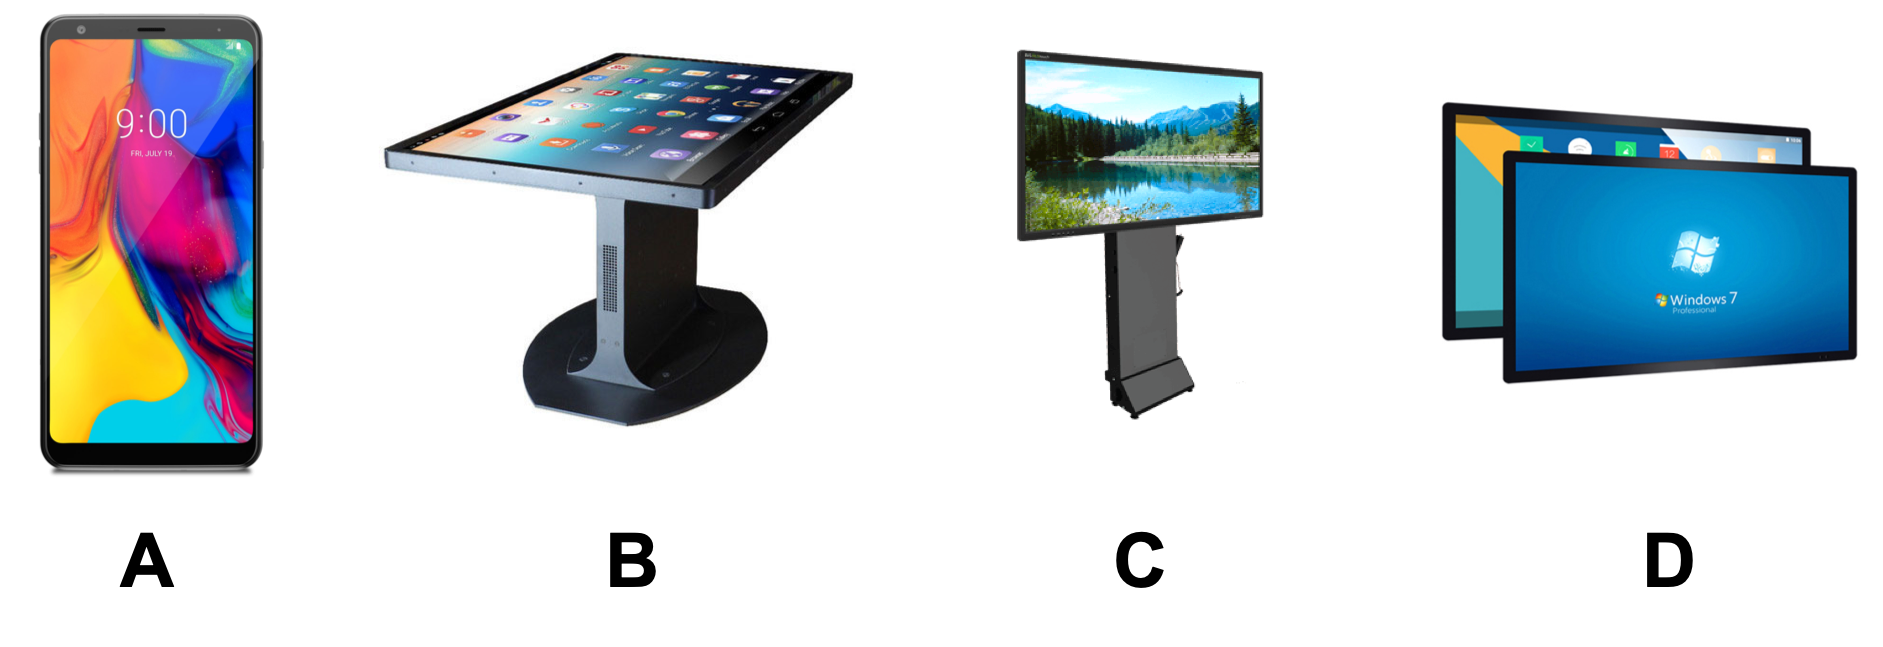
\includegraphics[width=0.8\columnwidth]{figures/touchproducts.png}
    \setlength{\belowcaptionskip}{-8pt}
    \caption{Capacitive touchscreen products: iphone (A). multitouch arcade touchscreen game table (B) interactive whiteboard (C). touchscreen Wall (D).}
    \label{fig:touchscreen-products}
  
\end{figure}

Researchers have explored enabling touch interfaces on everyday surfaces or objects ~\cite{Ono-Touch-and-Activate, Ono-2014,Sato-Touche, Xiao-WorldKit, Rekimoto-SmartSkin, olberding2013cuttable, Zhang-Electrick} with various sensing techniques. However, these prior work require dedicated sensing platforms such as Arduino to power touch interfaces and to enable wireless communication with digital devices. These requirements prevent end-users from easily fabricating customizable touch interfaces. As an alternative, researchers have proposed extending the capacitive sensing capability of the touchscreen to ambient surfaces through conductive strips. These systems can support interactions such as touch widgets ~\cite{Kato2015a,Kato2015,Kato2016}, trackpad ~\cite{mobicom-gao18} as well as tangible interfaces ~\cite{Schmitz2017, Schmitz2018, Chan-CapStones}. Unfortunately, these approaches can only support applications with very limited sensing range and fabrication materials. Furthermore, the sensing and fabrication methods, as well as the design space of long-range capacitive sensing beyond the touchscreen for interactive applications have not yet been studied. 

\begin{figure}
\centering
  \includegraphics[width=0.78\columnwidth]{figures/scenarios-ubicomp.png}
  \setlength{\belowcaptionskip}{-8pt}
  \caption{\textit{FlexTouch} supports various large-scale applications with different configurations. A: Discrete and 1-dimension touch widgets sensing long-range touch events. B: Fitness tracking using designs in A for the count of repetitions, distance and speed measurement on a treadmill, cycling and chest exercise machine. C: Body posture detection on the yoga mat with a built-in capacitive sensing matrix in an X-Y layout. D: Smart desk application for object presence and user's state detection. E. Smart mattress for sleep monitoring with a one-on-one mapping node matrix from the touchscreen.}
  \label{fig:scenarios}
  
\end{figure}
\section{Thesis Structure}
\section{Main Contributions}
In this paper, we present \textit{FlexTouch}, a technique for enabling long-range touch sensing interfaces beyond commercial touchscreens leveraging a variety of flexible conductive materials (Fig ~\ref{fig:scenarios}). \textit{FlexTouch} utilizes simple fabrication techniques to create a variety of passive, conductive 2D-patterned touch interfaces that enable new health and wellness applications. Our contributions in this paper are as follow:

1. We enabled large-scale touch sensing up to 4 meters and objects' presence up to 2 meters away from the capacitive touchscreen to ambient surroundings by including the local ground in the external conductive pattern design. 

2. We showed that \textit{FlexTouch} is easy to fabricate, assemble and use. The 2D circuit-like pattern is compatible with various conductive materials (copper foil tape, silver nanoparticle ink, ITO frames, and carbon paint), as well as fabrication methods (cutting, coating, and ink-jet printing). Furthermore, we proposed two easy attachment or assembly approaches to connect the extension part to touchscreens.  

3. We benchmarked the performance of \textit{FlexTouch} through user studies. Specifically, we fully explored design variables such as materials, extension strips' width as well as gap distance between strips and evaluated their impact on the coverage distance of \textit{FlexTouch}. In addition, we demonstrated the versatility and feasibility of \textit{FlexTouch} through applications such as body posture sensing, object presence detection as well as enhanced fitness sensing applications.
